\documentclass{mjw}
\title{Enforced Invariant Confluence}
\author{Michael Whittaker}

\usepackage[hidelinks]{hyperref}
\usepackage{amsfonts}
\usepackage[leqno]{amsmath}
\usepackage{amssymb}
\usepackage{amsthm}
\usepackage{centernot}
\usepackage{mathtools}
\usepackage{paralist}
\usepackage{python}
\usepackage{stmaryrd}
\usepackage{subcaption}
\usepackage{tikz}

\usetikzlibrary{arrows}
\usetikzlibrary{backgrounds}
\usetikzlibrary{calc}
\usetikzlibrary{decorations.pathmorphing}

% Implication.
\tikzstyle{impl}=[-implies, double distance=3pt]

% Transaction.
\tikzstyle{txn}=[ultra thick, ->]

% Derived transaction.
\tikzstyle{dtxn}=[ultra thick, ->, dashed]

% Invariant node.
\newcommand{\inode}[3][]{
  \node[draw, shape=circle, minimum width=0.5cm, #1] (#2) at (#3) {};
  \node[fill, shape=circle, #1] () at (#3) {};
}

% Normal node.
\newcommand{\nnode}[3][]{
  \node[fill, shape=circle, #1] (#2) at (#3) {};
}



\makeatletter
\newcommand{\leqnomode}{\tagsleft@true}
\newcommand{\reqnomode}{\tagsleft@false}
\makeatother

\newtheorem{theorem}{Theorem}
\renewcommand{\qedsymbol}{$\blacksquare$}
\newtheorem{claim}{Claim}
\renewcommand{\qedsymbol}{$\blacksquare$}

\newcommand{\figref}[1]{Figure \ref{fig:#1}}
\newcommand{\secref}[1]{Section \ref{sec:#1}}
\newcommand{\thmref}[1]{Theorem \ref{thm:#1}}
\newcommand{\clmref}[1]{Claim \ref{clm:#1}}

\newcommand{\defeq}{\stackrel{\mathclap{\normalfont\mbox{\scriptsize def}}}{=}}
\newcommand{\dom}[1]{\text{dom}}
\newcommand{\set}[1]{\left\{#1\right\}}
\newcommand{\denote}[1]{\left\llbracket#1\right\rrbracket}

\newcommand{\iinvariant}{\mathcal{I}}
\newcommand{\iconfluent}{$\iinvariant$-confluent}
\newcommand{\iconfluence}{$\iinvariant$-confluence}

\newcommand{\todo}[2][mwhittaker]{\textcolor{red}{TODO(#1): #2}}

\begin{document}
\maketitle

\reqnomode
\begin{abstract}
Strongly consistent systems are easy to reason about but face fundamental
limitations in availability and performance. Weakly consistent systems can be
implemented with very high performance but place a burden on the application
developer to reason about complex interleavings of execution.
\Invariantconfluence{} provides a formal framework for understanding when we
can get the best of both worlds. An \invariantconfluent{} object can be
efficiently replicated with no coordination needed to preserve its invariants.
However, actually determining whether or not an object is \invariantconfluent{}
is challenging: undecidable in general. In this paper, we establish conditions under
which a commonly used sufficient condition for \invariantconfluence{} is both
necessary and sufficient and use this condition to design (a) a general-purpose
interactive \invariantconfluence{} decision procedure and (b) a novel
sufficient condition that can be checked automatically. We then take a step
beyond \invariantconfluence{} and introduce a generalization of
\invariantconfluence{} called segmented \invariantconfluence{}, which allows us
to replicate non-\invariantconfluent{} objects with a small amount of
coordination. We implemented our theoretical findings in a prototype called
Lucy and found that our decision procedures efficiently handle common real-world workloads
including foreign key constraints, rollups, escrow transactions, and others.  We also
found that segmented \invariantconfluent{} replication can deliver up to an
order of magnitude more throughput than linearizable replication for low
contention workloads and comparable throughput for medium to high contention
workloads.
\end{abstract}

\section{Research Vision}

At a very high level, this research tackles the same problems tackled by many
existing research projects like BOOM Analytics \cite{alvaro2010boom}, Bloom
\cite{alvaro2011consistency}, Bloom$^L$ \cite{conway2012logic}, TARDiS
\cite{crookstardis}, and IPA \cite{holt2016disciplined}:

\begin{quotation}
  \emph{How can we make writing weakly consistent programs more principled?}
\end{quotation}

BOOM Analytics, Bloom, and Bloom$^L$ use data-centric declarative programming
and program analysis based on the CALM theorem. TARDiS exposes the entire
history of divergent computations to users in a git-like system to empower them
to programmatically resolve conflicts. IPA uses a type system to ensure weakly
consistent data doesn't leak into strongly consistent data. \todo{Cite and
summarize \cite{balegas2015putting}, \cite{roy2015homeostasis},
\cite{li2012making}, and \cite{li2014automating}}

This system builds off existing research on CRDTs and \iconfluence{} to provide
a library of CRDTs, a language to express invariants over those CRDTs, the
ability to transactionally update the replicated CRDTs, and a decision
procedure to algorithmically determine whether the transactions are
\iconfluent{} with respect to the invariants, ensuring coordination free
execution if they are and potentially giving illustrative counterexamples when
they are not. A simple example of psuedocode written with this system may look
something like this:

\begin{Python}
# Create an increment/decrement counter CRDT.
x = PNCounter(0)

# Set the invariant that the counter must always be non-negative.
set_invariant(x >= 0)

# This transaction is invariant confluent and would be accepted by the system.
@transaction
def foo():
  x.increment(42)

# This transaction is not invariant confluent and would be rejected by the
# system.
@transaction
def bar():
  x.decrement(1)
\end{Python}

A more complex example of psuedocode may look something like this:

\begin{Python}
# A map from employee id to employee name.
employees = Map[Int, String]()
# The number of employees.
num_employees = PNCounter(0)
# Employee ids partitioned into teams.
teams = Set[Set[Int]]

# The number of employees has to equal the size of employees.
set_invariant(num_employees = employees.size())
# All ids in teams must appear in employees.
set_invariant(forall team in teams. team subset employees.keys())
# All teams must be disjoint.
set_invariant(forall a, b in teams. a != b => a intersect b = {})
# Every employee must be on a team
set_invariant(union(teams) = employees.keys())

# This transaction which adds a new employee would be checked for
# invariant-confluence by the system.
@transaction
def add_employee(name):
  id = employees.unique_id()
  employees.put(name, id)
  num_employees.increment(1)
  teams[0].add(id)
\end{Python}

This pseudocode brings up a lot of \emph{theoretical questions}...
\begin{inparaitem}
  \item What CRDTs and what operations can we support?
  \item What invariant languages can we support?
  \item Given the set of CRDTs and invariants, is determining invariant
    confluence even decidable?
  \item If so, can it be determined efficiently?
  \item If not, how can we limit the CRDTs, operations, or invariants to make
    it decidable?
\end{inparaitem}
...and a lot of \emph{systems questions}:
\begin{inparaitem}
  \item Is the system expressive enough to write real-world programs?
  \item Can the system be implemented as a library in an existing programming
    language?
  \item How do we architect and build an actual system out of this?
\end{inparaitem}

This research aims to answer these questions and develop a first-of-its-kind
system that allows programmers to write coordination free distributed systems
with more discipline than ever before.

\section{Counters}
As a first step towards accomplishing our research vision, let's begin with a
\emph{simple} CRDT with \emph{simple} operations and a \emph{simple} invariant
language: PN-counters and linear equations and inequalities.

\subsection{Overview}
Recall that a \emph{G-Counter} CRDT is an increment-only counter
\cite{shapiro2011comprehensive}. A state-based G-Counter distributed across $n$
machines $1, 2, \ldots, n$ can be implemented as an $n$-tuple $(x_1, x_2,
\ldots, x_n)$ of natural numbers. The \emph{increment($k$) method} at machine
$i$ increments $x_i$ by $k$; the \emph{query method} returns the sum of the
tuple $\sum_{i=1}^n x_i$; and the \emph{merge method} computes the pairwise max
of two $n$-tuples.

A \emph{PN-Counter} CRDT is a counter which supports increments and decrements
and can be implemented as a pair $(p, n)$ of two G-Counters
\cite{shapiro2011comprehensive}. increment($x$) increments $p$ by $x$;
decrement($x$) increments $n$ by $x$; query returns $p - n$; and merge performs
a pairwise merge of $p$ and $n$.

Our \emph{invariant language} is formed from \emph{linear equations} (e.g. $x =
0$, $2x = y$, $-x + 42y - 2z = 16$) and \emph{inequalities} (e.g. $x > 0$, $2x
\leq y$, $-x + 42y - 2z \neq 16$) connected with the boolean connectives
\emph{and} ($\land$), \emph{or} ($\lor$), and \emph{not} ($\lnot$) (e.g.
$\lnot((\lnot(x < 0) \lor 2x = y) \land -x + 42y - 2z \geq 16)$).

A \emph{transaction} chooses a subset of variables and decrements or increments
each by a constant amount. For example, a transaction may increment $x$ by 1,
decrement $y$ by 42, and increment $z$ by 100.

Given a set of transactions and an invariant, we want to determine whether the
transactions are \iconfluent{} with respect to the invariant. For example, the
transaction that \emph{increments} $x$ by 1 is invariant confluent with respect
to the invariant $x > 0$, but the transaction that \emph{decrements} $x$ by 1
is not, as shown in \figref{decrement}.

\begin{figure}[h]
  \centering
  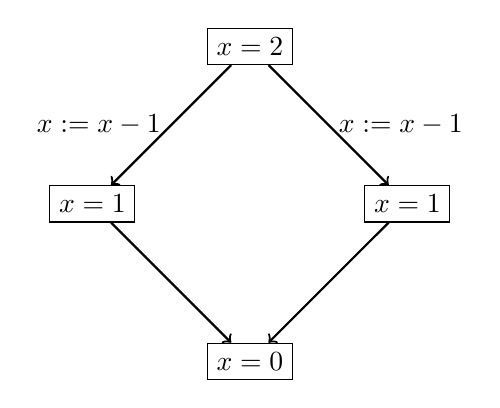
\begin{tikzpicture}
    % \draw (0, 0) grid (4, 4);
    \node[draw] (start)  at (2, 4) {$x=2$};
    \node[draw] (left)   at (0, 2) {$x=1$};
    \node[draw] (right)  at (4, 2) {$x=1$};
    \node[draw] (merged) at (2, 0) {$x=0$};

    \draw[thick, ->] (start) to node[left]  {$x := x - 1$} (left);
    \draw[thick, ->] (start) to node[right] {$x := x - 1$} (right);
    \draw[thick, ->] (left)  to (merged);
    \draw[thick, ->] (right) to (merged);
  \end{tikzpicture}
  \caption{
    A counterexample showing transaction $x := x - 1$ is not invariant
    confluent with respect to the invariant $x > 0$. The top, left, and right
    states satisfy the invariant, but the bottom state does not.
  }
  \label{fig:decrement}
\end{figure}

\subsection{Formalizing the Question}
\newcommand{\var}{\textsf{Var}}
\newcommand{\ints}{\mathbb{Z}}

Our invariant language is defined by the grammar in \figref{invariant-grammar}
which includes linear equations and inequalities over variables in a finite set
$\var$ and integer constants in $\ints$.

\begin{figure}[h]
  \centering

  \newcommand{\atom}{\textsf{atom}}
  \newcommand{\aexp}{\textsf{aexp}}
  \newcommand{\bexp}{\textsf{bexpr}}
  \begin{gather*}
    \begin{array}{rrll}
      \atom & ::= & k & \text{\emph{constants}} \\
            & |   & x & \text{\emph{variables}} \\
      &&& \\
      \aexp  & ::= & \atom         & \text{\emph{atom}} \\
             & |   & -\atom        & \text{\emph{negation}} \\
             & |   & \aexp + \aexp & \text{\emph{addition}} \\
             & |   & \aexp - \aexp & \text{\emph{subtraction}} \\
      &&& \\
      \bexp  & ::= & \aexp \leq \aexp  & \text{\emph{inequality}} \\
             & |   & \lnot \bexp       & \text{\emph{negation}} \\
             & |   & \bexp \land \bexp & \text{\emph{conjunction}} \\
             & |   & \bexp \lor \bexp  & \text{\emph{disjunction}} \\
    \end{array}
  \end{gather*}

  \caption{
    A grammar for our linear equation and linear inequality invariant language.
    Note that the comparison operators $=$, $\neq$, $<$, $>$, and $\geq$ are
    not included because they can be defined in terms of the existing
    operators.
  }
  \label{fig:invariant-grammar}
\end{figure}

A \emph{database state} is a total function $D: \var \to \ints$.  We say a
database state $D$ \emph{satisfies invariant} $I$ if $I$ evaluates to true
after all variables in $I$ have been replaced by their mapping in $D$.

A \emph{transaction} is a partial function $t: \var \rightharpoonup \ints$.
\emph{Applying a transaction} $t$ to database state $D$, denoted by $D \circ
t$, produces a new database state defined as follows:
\[
  (D \circ t)(x) \defeq \begin{cases*}
    D(x) + t(x) & $x \in \dom{}(t)$ \\
    D(x)        & otherwise
  \end{cases*}
\]
Note that transaction application is commutative. That is for all database
states $D$ and transactions $t_1$ and $t_2$, $D \circ t_1 \circ t_2 = D \circ
t_2 \circ t_1$.

A transaction chain $C$ created from a set of transactions $T$ is a sequence of
transactions $t_1, \ldots, t_n$ where $t_j \in T$ for $1 \leq j \leq n$. Let $D
\circ C$ be syntactic sugar for $D \circ t_1 \circ \cdots \circ t_n$. We say
$C$ \emph{satisfies invariant} $I$ starting at $D$ if for every prefix $C'$ of
$C$, $D \circ C'$ satisfies invariant $I$.

A set of transactions $T$ is \iconfluent{} with respect to invariant $I$ if for
all database states $D$ and chains $C_1$ and $C_2$ created from $T$, if $D$
satisfies $I$, $C_1$ satisfies $I$ starting at $D$, and $C_2$ satisfies $I$
starting at $D$, then so does $D \circ C_1 \circ C_2$.

\subsection{A Geometric Interpretation}
\newcommand{\inva}{x + y \geq 0}
\newcommand{\invb}{x - y \leq 0}
\newcommand{\invc}{x \geq 1}
\newcommand{\invd}{x \geq 3}
\newcommand{\inv}{(\inva \land \invb \land \invc) \lor (\invd)}

Sometimes, we can eyeball whether a transaction is \iconfluent{} with respect
to an invariant. Other times, not so much. For example, which transactions are
invariant confluent with respect to the invariant $\inv$? It's not immediately
clear.  Surprisingly, we can interpret the question ``Is $T$ \iconfluent{} with
respect to $I$?'' geometrically, and doing so will make answering the question
much easier!

Consider an invariant $I$ over $n$ variables $x_1, \ldots, x_n$. If we imagine
the values of the $n$ variables as an $n$-dimensional point, then we can draw
the set of points in $\ints^n$ that satisfy $I$. In fact, if we canonicalize
$I$ by eliminating negations and converting to conjunctive normal form, then
the set of points satisfying $I$ is the intersection (for $\land)$ and union
(for $\lor$) of the solutions to a set of linear equations and inequalities,
which is always straightforward to draw. For example, the set of points
satisfying $\inv$ is shown in \figref{geometric-example}.

\begin{figure}
  \newenvironment{griddedpic}{
    \begin{tikzpicture}
      \clip (-4, -1) rectangle (4, 4);
  }{
      \draw (-4, -1) grid (4, 4);
      \draw[ultra thick] (-4, 0) -- (4, 0);
      \draw[ultra thick] (0, -1) -- (0, 4);
    \end{tikzpicture}
  }

  \begin{subfigure}[c]{0.5\textwidth}
    \begin{griddedpic}
      \fill[red, opacity=0.4]
        (-10, 10) -- (10, -10) -- (10, 10) -- cycle;
    \end{griddedpic}
    \caption{$\inva$}
  \end{subfigure}
  \begin{subfigure}[c]{0.5\textwidth}
    \begin{griddedpic}
      \fill[blue, opacity=0.4]
        (-10, -10) -- (10, 10) -- (-10, 10) -- cycle;
    \end{griddedpic}
    \caption{$\invb$}
  \end{subfigure}

  \vspace{0.5cm}

  \begin{subfigure}[c]{0.5\textwidth}
    \begin{griddedpic}
      \fill[green, opacity=0.4]
        (-10, 1) -- (10, 1) -- (10, 10) -- (-10, 10) -- cycle;
    \end{griddedpic}
    \caption{$\invc$}
  \end{subfigure}
  \begin{subfigure}[c]{0.5\textwidth}
    \begin{griddedpic}
      \fill[orange, opacity=0.4]
        (-10, 3) -- (10, 3) -- (10, 10) -- (-10, 10) -- cycle;
    \end{griddedpic}
  \caption{$\invd$}
  \end{subfigure}

  \vspace{0.5cm}

  \begin{subfigure}[c]{\textwidth}
    \centering
    \begin{griddedpic}
      \fill[purple, opacity=0.4]
        (-1, 1) -- (-3, 3) -- (-10, 3) -- (-10, 10) -- (10, 10) -- (10, 3) --
        (3, 3) -- (1, 1) -- cycle;
    \end{griddedpic}
    \caption{$\inv$}
  \end{subfigure}

  \caption{An illustration of the solution to $\inv$.}
  \label{fig:geometric-example}
\end{figure}

Next, we can imagine a transaction $t$ as an $n$-dimensional vector $(k_{x_1},
\ldots, k_{x_n})$ where $t$ adds constant $k_{x_i}$ to variable $x_i$. Now, the
question of whether a set of transactions $T$ is \iconfluent{} with respect to
invariant $I$ has been reduced to the following question. Starting at an
arbitrary point $D$ in the solution space of $I$, if we can add vectors $t^1_1,
t^1_2, \ldots, t^1_m$ to $D$ and vectors $t^2_1, t^2_2, \ldots, t^2_n$ to $D$
all while staying in the solution space of $I$, then are we guaranteed that $D
+ t^1_1 + t^1_2 + \ldots + t^1_m + t^2_1 + t^2_2 + \ldots + t^2_n$ is in the
solution space of $I$?

Turning again to our example in \figref{geometric-example}, it is now clear
that any transaction $(k_x, k_y)$ where $y \geq 0$ and $|x| \leq y$ is
\iconfluent{} with respect to $\inv$. These are the vectors that point up and
not too far left or right.

\subsection{One is Enough}
Define a set of transactions $T$ to be $k$-\iconfluent{} with respect to
invariant $I$ if for all database states $D$ and chains $C_1$ and $C_2$ created
from $T$ of length at most $k$, if $D$ satisfies $I$, $C_1$ satisfies $I$
starting at $D$, and $C_2$ satisfies $I$ starting at $D$, then so does $D \circ
C_1 \circ C_2$.
%
A set of transactions $T$ is \iconfluent{} with respect to an invariant $I$ if
it is $k$-\iconfluent{} for all $k$. Thus, when reasoning about \iconfluent{}
transactions, we have to consider potentially large transaction chains which
can be a bit brain boggling. Reasoning about 1-\iconfluence{} is much easier
because we only have to consider a pair of transactions at a time. This
subsection proves a convenient lemma that 1-\iconfluence{} and \iconfluence{}
are equivalent.

\begin{theorem}
  For all sets of transactions $T$ and invariants $I$, T is 1-\iconfluent{} if
  and only if it is \iconfluent{}.
\end{theorem}
\begin{proof}
  The reverse direction is immediate from the definition of \iconfluence{}. For
  the forward direction, consider a set of transactions $T$ that is
  1-\iconfluent{} with respect to an invariant $I$, but assume for
  contradiction that $T$ is not \iconfluent{} with respect to $I$. That is,
  there exists a database state $D$ and two chains $C^1 = t^1_1, t^1_2, \ldots,
  t^1_m$ and $C^2 = t^2_1, t^2_2, \ldots, t^2_n$ such that $D$ satisfies $I$,
  $C^1$ satisfies $I$ starting at $D$, and $C^2$ satisfies $I$ starting at $D$
  but $D \circ C^1 \circ C^2$ does not.

  Let $C^z_j$ denote the prefix of $C^z$ of length $j$. We show by strong
  mathematical induction on $i$, that $D \circ C^1_j \circ C^2_k$ satisfies $I$
  for all $0 \leq j \leq m$, $0 \leq k \leq n$, and $0 \leq i = j + k \leq n +
  m$.
  %
  The base case, when $i = 0$, is trivial. $j = k = 0$, and $D \circ C^1_0
  \circ C^2_0 = D$ which satisfies $I$ by assumption.
  %
  For the inductive step, we wish to show for arbitrary $0 \leq j \leq m$, $0
  \leq k \leq n$, and $0 < i = j + k$ that $D \circ C^1_j \circ C^2_k$
  satisfies $I$. If $j = 0$, then $D \circ C^1_0 \circ C^2_k = D \circ C^2_k$
  satisfies $I$ by the assumption that $C^2$ satisfies $I$ starting at $D$, and
  likewise for when $k = 0$. Now consider $j, k > 0$. By the inductive
  hypothesis, we know
    (1) $D \circ C^1_{j-1} \circ C^2_{k-1}$,
    (2) $D \circ C^1_{j-1} \circ C^2_{k}$, and
    (3) $D \circ C^1_{j}   \circ C^2_{k-1}$
  all satisfy $I$. If we let (1) be our initial database state, $t^1_j$ be one
  chain, and $t^2_k$ be the other chain, then the 1-\iconfluence{} of $T$ tells
  us that $(1) \circ t^1_j \circ t^2_k = D \circ C^1_j \circ C^2_k$ satisfies
  $I$.
\end{proof}


\pagebreak{}
\bibliography{bib}
\bibliographystyle{plain}
\end{document}
